\documentclass{article}
\usepackage{amsmath}
\usepackage[utf8]{inputenc}
\usepackage{graphicx}
\graphicspath{ {Figures/} }


\newcommand{\HeatingDegreeDays}{\mbox{HDD}}
\newcommand{\BalancePointTemperature}{\mbox{BPT}}
\newcommand{\Temperature}{\mbox{T}}
\newcommand{\NormalDemand}{\mbox{Normal Demand}}
\newcommand{\ActualDemand}{\mbox{Actual Demand}}
\newcommand{\TotalDemand}{\mbox{Total Demand}}
\newcommand{\NormalHDD}{\mbox{Normal HDD}}
\newcommand{\ActualHDD}{\mbox{Actual HDD}}
\newcommand{\StandardAdjustment}{\mbox{Standard Adjustment}}
\newcommand{\TemperatureSensitiveUse}{\mbox{Temperature Sensitive Use}}
\newcommand{\BaseLoad}{\mbox{Base Load}}

\newcommand{\eqPeriod}{\,.}
\newcommand{\eqComma}{\,,}
\newcommand{\Farenheit}[1]{{#1}$^o$F}


\title{Forecasting Design Day Demand Using Extremal Quantile Regression}
\author{David J. Kaftan, Jarrett L. Smalley, George F. Corliss, \\
Ronald H. Brown, and Richard J. Povinelli \\
GasDay Project, Marquette University, Milwaukee, WI
}
\date{}

\begin{document}

\maketitle

\begin{abstract}
Extreme events occur rarely, making them difficult to predict. Extreme cold events strain natural gas systems to their limits. Natural gas distribution companies need to be prepared to satisfy demand on any given day that is at or warmer than an extreme cold threshold. The hypothetical day with temperature at this threshold is called the Design Day. To guarantee Design Day demand is satisfied, distribution companies need to determine the demand that is unlikely to be exceeded on the Design Day.

We approach determining this demand as an extremal quantile regression problem. We review current methods for extremal quantile regression. We implement a quantile forecast to estimate the demand that has a minimal chance of being exceeded on the design day. We show extremal quantile regression to be more reliable than direct quantile estimation. We discuss the difficult task of evaluating a probabilistic forecast on rare events.

Probabilistic forecasting is a quickly growing research topic in the field of energy forecasting. Our paper contributes to this field in three ways. First, we forecast quantiles during extreme cold events where data is sparse. Second, we forecast extremely high quantiles that have a very low probability of being exceeded. Finally, we provide a real world scenario on which to apply these techniques.    
\end{abstract} 

{\bf Index terms: Energy demand, natural gas demand, extremal quantile regression}

\section{Introduction}
%background of ng forecating, importance, extreme events...
Natural gas Local Distribution Companies (LDCs) need to provide steady flow to their customers. It is important for these LDCs to be able to forecast future demand, as to be able to reserve and send out an appropriate amount of natural gas. With a large portion of natural gas usage being for spatial heating, natural gas Demand is highly weather dependent \cite{vitullo2009mathematical}. Extreme cold events stress the limits of the distribution system, as this is often when natural gas demand is at its maximum. The Design Day is the hypothetical day when temperatures break a given extreme cold threshold. The Design Day condition is the temperature of an extreme event that only occurs once in n years. The Design Day demand is the natural gas demand that is forecasted to occur on a day with the Design Day condition. This is the demand that the LDC should be able to supply up to. 

Probabilistic forecasting methods offer an appropriate model to forecast extreme events, since they are characterized as only happening once in n years. Probabilistic forecasts of extreme events are advantageous as they reflect the inherent uncertainty of extreme event forecasting, while giving forecast end users the information needed to make system-wide decisions \cite{murphy1991probabilities}.


\section{Background}

%extremal quantile regression
Quantile regression is a method for predicting the cumulative density function of a response variable conditional on a predictor variable \cite{koenker1978regression}. For example, quantile regression can answer the question: what is the demand that has 10 percent chance of being exceeded if the temperature is 20 \textsuperscript{o}F? The relationship between the response variable and the predictor variable for a given quantile (i.e., 10 percent chance of being exceeded) can be found by minimizing the pinball loss function - typically through linear programming methods.

Problems arise when we choose an extremely high (or low) quantile. Consider the situation where we want to predict the demand that will be exceeded 0.01 percent of the time for a given temperature. Perhaps we only have 100 data points on which to fit this relationship. That means we are fitting a line above every data point in our data set. In this case, using traditional quantile regression will not give us reasonable results. Extremal Quantile Regression extends the concept of quantile regression to the extreme tails of a distribution \cite{chernozhukov2005extremal}. One particularly useful method is introduced by Wang \cite{wang2012estimation}. The conditional relationship is assumed to be the same across higher quantiles. For example, the conditional relationship between demand and temperature is the same for the 90\textsuperscript{th} and 99\textsuperscript{th} quantiles. The only difference between these two quantiles is constant with temperature (i.e., a bias term). The bias term is determined using extreme value theory.

\section{Methods}

We estimate the $99.38^{th}$ quantile of flow, given temperature. This quantile is requested by our customers and corresponds to 2.5 standard deviations above the mean of a normal distribution. We start with a quantile regression model of demand and temperature, making the following four adjustments. First, we address the non-linear relationship between temperature and flow. Second, we account for our desire for performance during extreme cold days. Third, we address the challenge of modeling an extremely high quantile. Fourth, we account for the long term out of sample uncertainty.

\subsection{Non-Linear relationship between Temperature and Flow}

As seen in Figure 1, there is a non-linear relationship between temperature and flow. Typically, this relationship is accounted for by transforming temperature into heating degree days (HDD), based on a reference temperature, 
\begin{equation}
    HDD= \mbox{max}(0, T_{Reference}-T_{Current})~.
    \label{eqn:hdd}
\end{equation}

\begin{figure} \label{fig:scatterTempAndFlow}
	\centering
	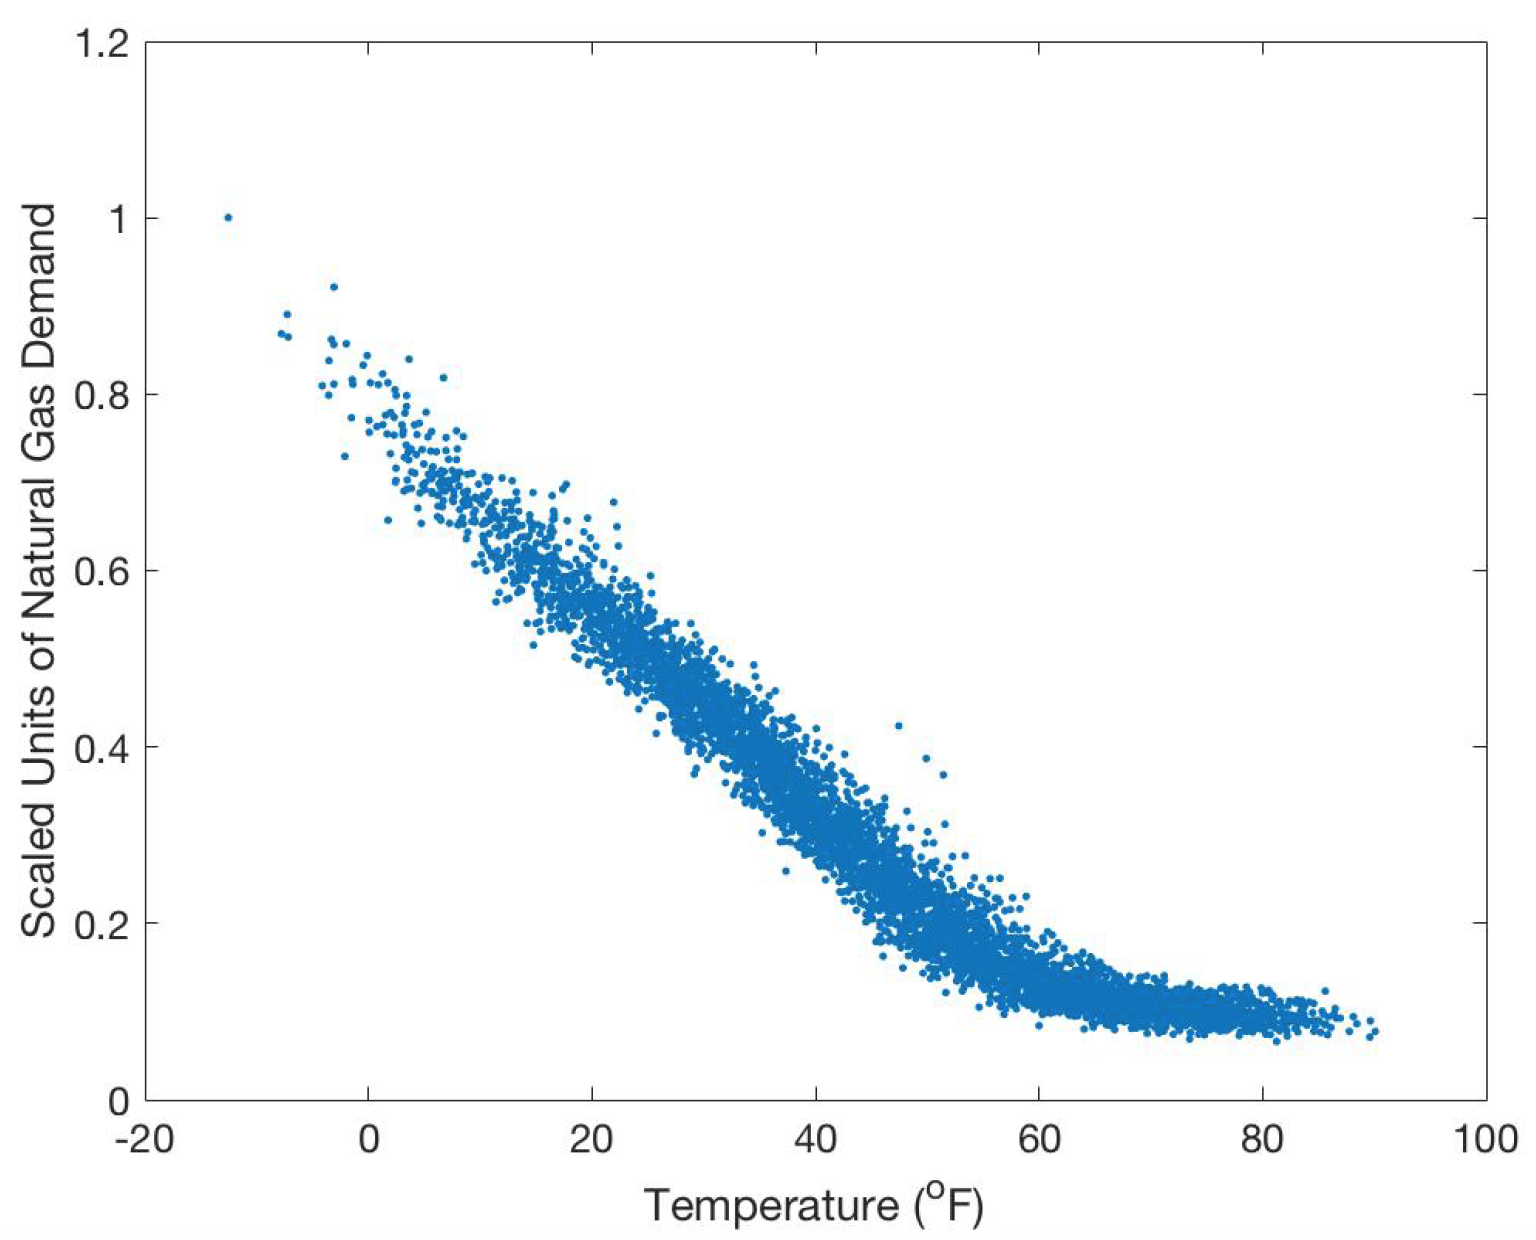
\includegraphics[scale=0.4]{nonlinear.png}
	\caption{Demand is non-linear with temperature. However, when temperature is less than 65 \textsuperscript{o}F, demand is approximately linear.}
\end{figure}

Heating degree days allow us to assume temperature independence from flow at warm temperatures and linear temperature dependence at colder temperatures. However, it does not account for the bias shift in uncertainty around 65 degrees F. Rather than using an indicator variable to represent temperatures colder than 65 degrees F, we ignore all temperatures warmer than 50 degrees F. Conveniently, in our analysis of design day conditions, we are only concerned about the coldest temperatures, so removing the warm temperatures inquires no loss.

\subsection{Performing Well on Cold Days}

After removing the warm days, we have significantly less data. We would like to model the demand on the coldest days, but we lack enough data to do so. We assume the remaining data can give us information about demand on the coldest days, but we know that our coldest data is best. We therefore weigh the pinball loss by temperature in the quantile regression optimization. This is done by sorting the pinball loss vector by temperature (the first index is the warmest temperature) and adjusting each element $i$ in the vector of length $N$ accordingly:

\begin{equation}
    AdustedPinball_i = SortedPinball_i \times (1 + \frac{i}{N}).
\end{equation}

The adjusted pinball loss on the coldest day is now weighted twice as heavy as the warmest day. When minimizing the adjusted pinball loss, a quantile will be fit better to the coldest days. These weights are visualized in Figure 2.

\begin{figure} \label{fig:weighting}
	\centering
	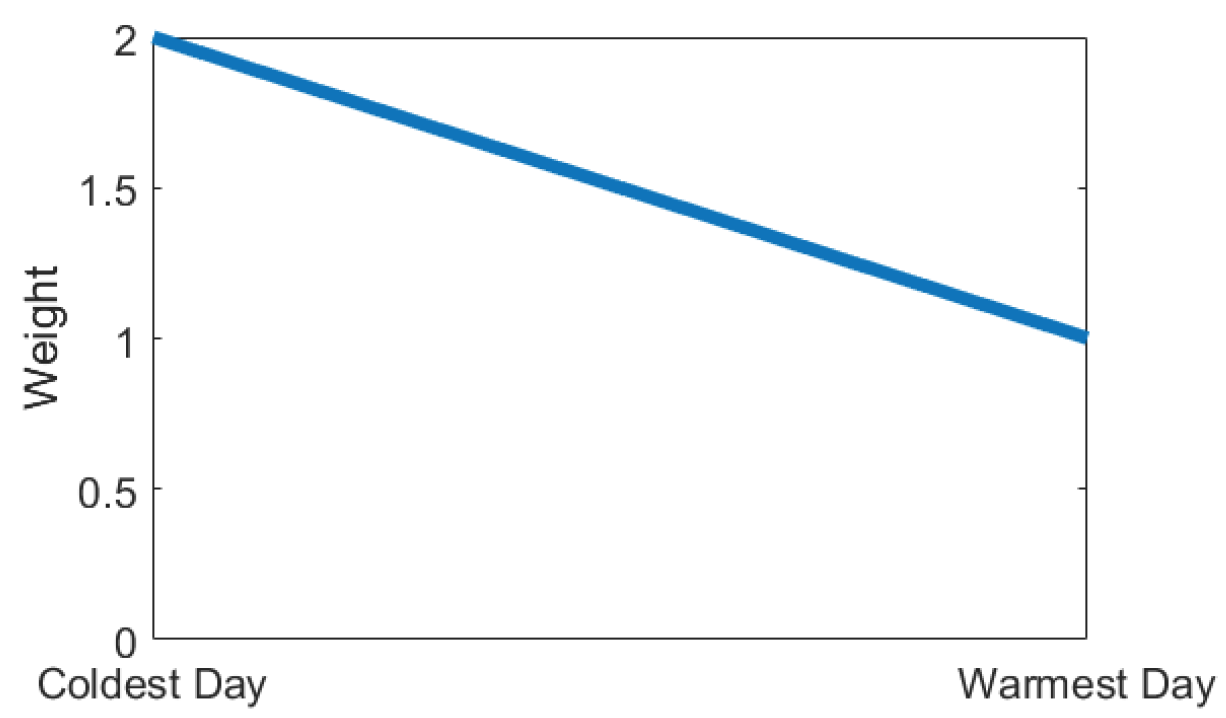
\includegraphics[scale=0.4]{weighting.png}
	\caption{Weighting of pinball loss optimization}
\end{figure}

\subsection{Estimating Extreme High Quantiles}

When estimating in the extreme quantiles, results can be very unexpected and even unindicative of the underlying distribution. At high enough quantiles with little data, quantile regression will fit a line through the two most extreme outliers (given a 2 parameter model). We have already begun to mitigate this by weighting the optimization of the coldest points rather than removing non-extreme cold data. We further account for this by using composite quantile regression (also known as weighted quantile regression, or Hogg's method \cite{koenker2004quantile}). Consider a two parameter linear model relating the 99.38\textsuperscript{th}, 91.88\textsuperscript{th}, and 84.38\textsuperscript{th} quantiles of flow to heating degree days and a bias term. Composite quantile regression allows us to estimate the temperature parameter using all three quantiles, leaving only the bias parameter to be determined for the extreme high quantile. The resulting estimates for the three quantiles are the parallel lines shown in Figure \ref{composite}.

\begin{figure}
	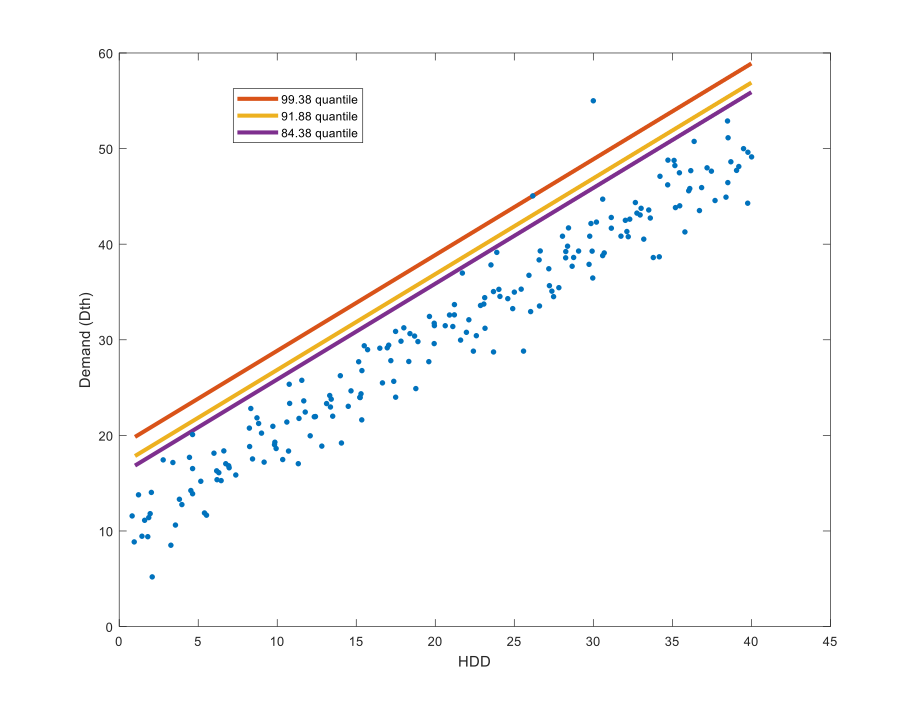
\includegraphics[scale=0.7]{composite.png}
	\caption{Result of using composite quantile regression using simulated data}\label{composite}
\end{figure}

\subsection{Long Term Out Of Sample Uncertainty} \label{longterm}

It is well known that errors are often greater for out-of-sample testing than for in-sample testing. Since we are forecasting the quantile for the following year, we need to adjust based on out-of-sample uncertainty \cite{DKaftan2018}. We start with the same 2 parameter (HDD and bias terms) linear model for the 99.38\textsuperscript{th} quantile. We first train (detrend data \cite{brown2015detrending} and perform quantile regression) our model on a single year of data. We then validate on a single year of data and re-fit the bias term based on the residuals. We record the change in the bias term from the training data to the validation data. This process is repeated using the first two years as a training set and the third as a validation set, then again until the last year of training data is used as the validation set. We determine the mean absolute change of the bias term. Finally, we fit a model to all of the training data. We add the mean absolute change to the bias term in order to account for the out-of-sample uncertainty.

\section{Results}

The experiment is run on the 100 most temperature-sensitive datasets GasDay forecasts. The experiment is run in two folds. First, we hold out the 2017 heating season for testing, and we train on all previous years. Second, we hold out the 2016 heating season for testing and train on all previous years.

Our experiment reflects our goal; we need to estimate the quantile representing demand that is exceeded 0.62\% (100\% - 99.38\%) of days in a heating season. We therefore count the number of exceedances of the quantile in the test set. In particular, we want to perform well during the coldest days in winter. We therefore limit our analysis to the 10\% coldest days of the test set, as seen in Figure \ref{qrResults}.
\begin{figure}
	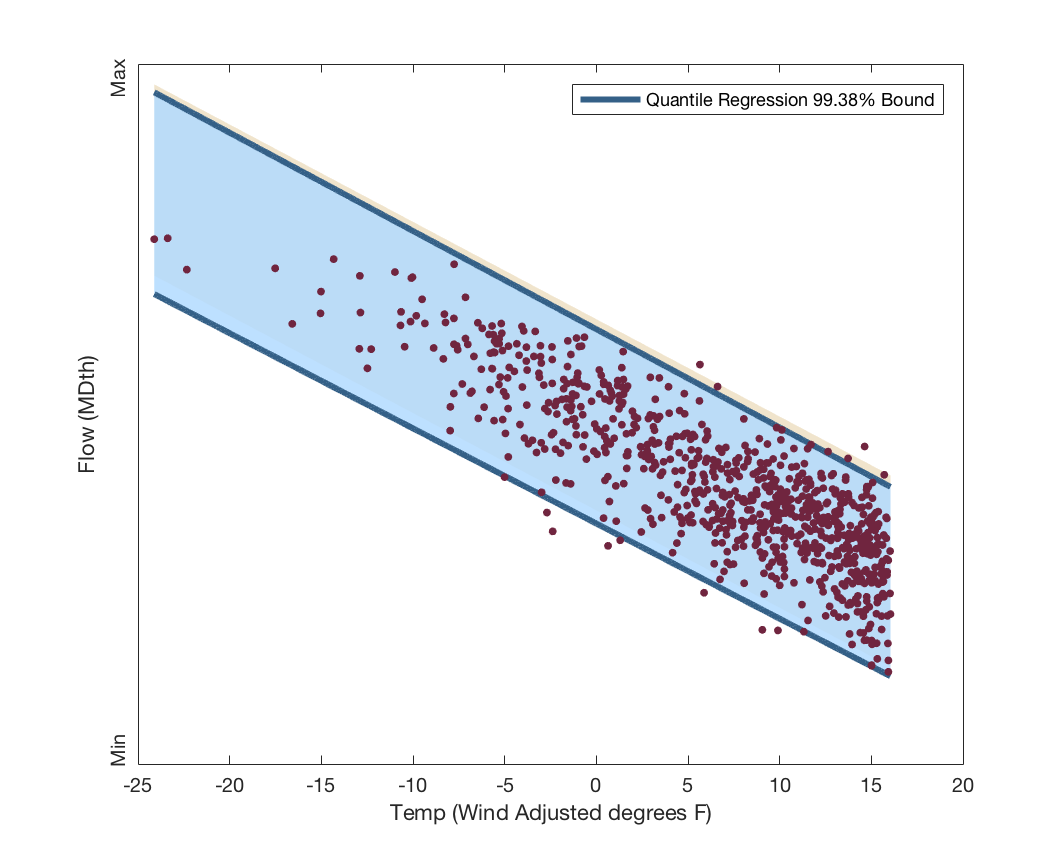
\includegraphics[scale=0.3]{bienLab3.png}
	\caption{Anonymized fit of the 99.38\textsuperscript{th} and 0.62\textsuperscript{th} quantiles on the coldest days}\label{qrResults}
\end{figure}
 Across the two test folds, we expect 44.70 exceedances. In total, our method incurs 38 exceedances: 85.0\% of the expected exceedances. For the sake of evaluating the strategy for dealing with long-term out of sample uncertainty described in Section \ref{longterm}, we evaluated our experiment absent of said strategy. The result showed our bounds unreasonably tight with over 200\% of the expected exceedances.

\section{Conclusion}

This work introduces an interesting problem to the forecasting community: forecasting the Design Day demand. Using methods common in forecasting literature - along with novel extensions - we are able to successfully predict the demand that is extremely unlikely to be exceeded during the Design Day. 



\bibliographystyle{ieeetr}

\bibliography{references}
\end{document}